\subsection{写真撮影画面}
写真撮影画面ではiPhoneに内蔵されているカメラを使用して観光スポットの写真を撮影する。カードリスト画面で木古内の魅力を知り、実際に観光スポットを訪れたユーザにそこを訪れた記念を残してもらうために写真を撮ってもらう。撮った画像はカードリストの画像に上書きされ、表示される。カードリスト画面のカメラボタンをタップすることで写真撮影画面に遷移する。写真撮影画面を図6.3(a)で示す。画面の下の中央にある丸いボタンをタップすると写真を撮ることができる。左下の「キャンセル」ボタンをタップすると写真撮影画面からカードリスト画面に遷移する。左上のボタンによりフラッシュの有無を選択でき、暗い風景を撮るときなどに使用する。右上のボタンはインカメラとアウトカメラの切り替えを行うことができる。写真撮影後、その画像を保存するか選択する写真保存画面に遷移する。写真保存画面を図6.3(b)で示す。写真保存画面ではユーザが撮った写真を保存したい場合、右下の「写真を使用」ボタンをタップすることでその写真は保存され、撮った場所に対応するカードに表示される。写真を撮り直す場合は、左下の「再撮影」ボタンをタップすることで写真撮影画面に戻ることができる。
\newpage

\begin{figure}[htbp]
  \begin{center}
    \begin{tabular}{c}

      % 1
      \begin{minipage}{0.33\hsize}
        \begin{center}
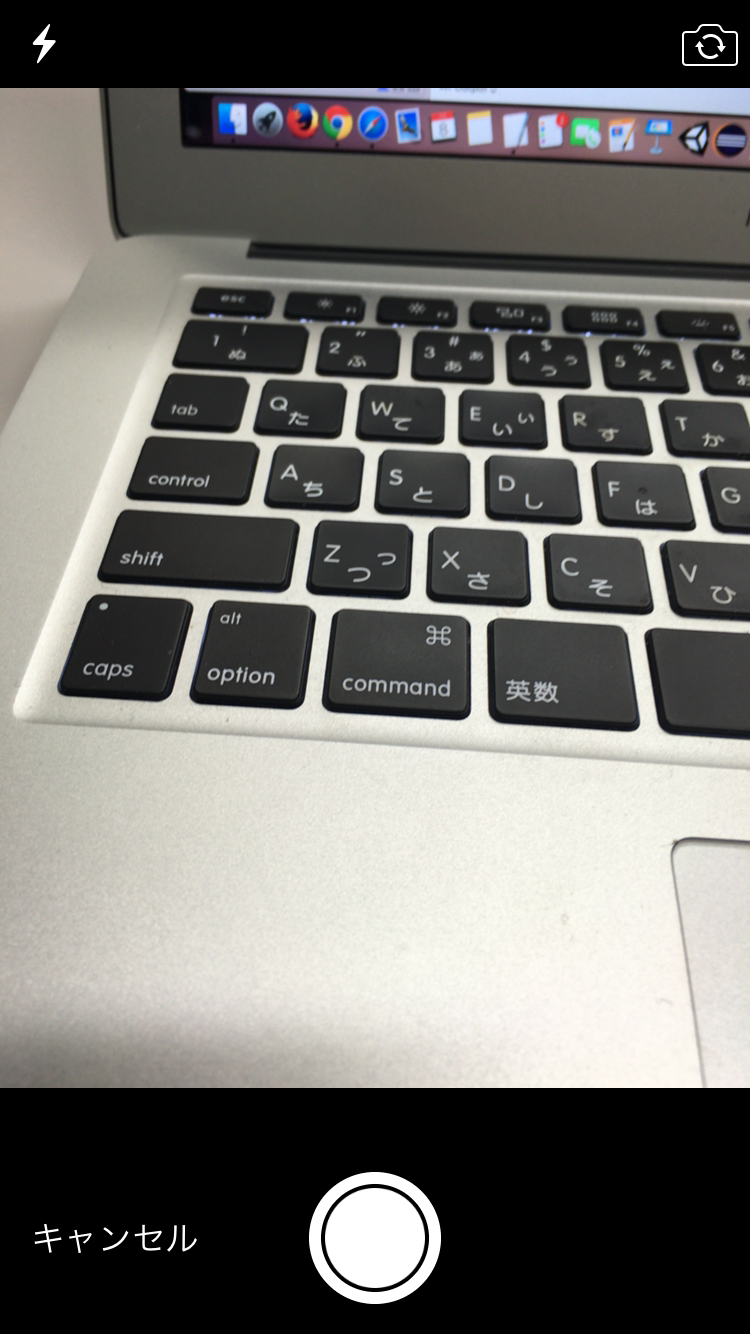
\includegraphics[width=4cm, bb=0 0 304 570]{kiko_takephoto1.PNG}
          \hspace{1cm} (a)写真撮影画面
        \end{center}
      \end{minipage}

      % 2
      \begin{minipage}{0.33\hsize}
        \begin{center}
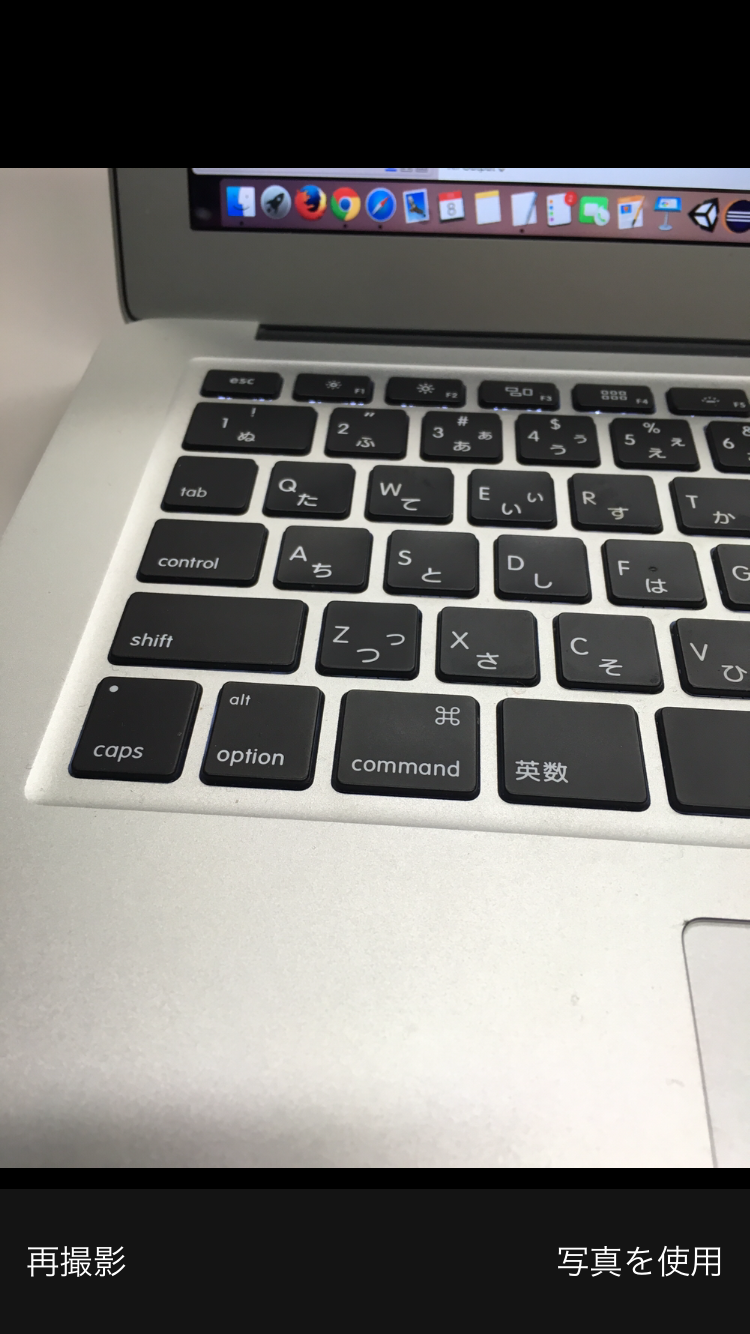
\includegraphics[width=4cm, bb=0 0 304 570]{kiko_takephoto2.PNG}
          \hspace{1cm} (b)写真保存画面
        \end{center}
      \end{minipage}
      
    \end{tabular}
    \caption{写真を撮影する機能の画面}
    \label{fig:lena}
  \end{center}
\end{figure}          

\bunseki{池田俊輝}